\section{Appendix}

\subsection{Over het Begrip Afgeleide}\label{sec:appafg}

In de inleiding zagen we dat de marginale opbrengst en de marginale kost respectievelijk de opbrengst en de kost zijn \textit{van de laatste of volgende eenheid}. Koopt men per product, bijvoorbeeld per appel, dan gaat dit over de opbrengst of kost van de laatst gekochte appel. Stelt men - ter illustratie - een staafjesdiagram op met de totale kost bij stijgende hoeveelheid appelen, dan is de marginale kost van de vijfde appel gewoon wat men meer zal moeten betalen om - na vier appelen te hebben gekocht - een vijfde appel te kopen. Dit valt af te lezen in figuur \ref{fig:appendix1} : het is de stijging van het laatste balkje. \\

\begin{figure}[H]
\centering
\captionsetup{justification=centering,margin=2cm}
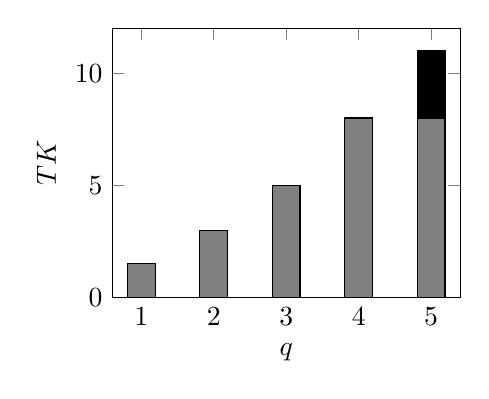
\begin{tikzpicture}
	\begin{axis}[xlabel=$q$, ylabel=$TK$, ymin=0,xtick={1,...,5}, ymax=12, width=6cm, height=5cm]
		\addplot[ybar,fill=black] coordinates {(5,11)};
		\addplot[ybar,fill=gray] coordinates {(1,1.5)(2,3)(3,5)(4,8)(5,8)};
	\end{axis}
\end{tikzpicture}
\caption{De totale kost van een bepaalde hoeveelheid appelen, \\met in het zwart de marginale kost van de vijfde appel}
\label{fig:appendix1}
\end{figure}

\par Is de hoeveelheid $q$ van het product echter continu ($q$ kan alle positieve waarden aannemen, men koopt bijvoorbeeld per kilo), dan worden de zaken iets ingewikkelder. Als je dan de totale opbrengst $TO$ of de totale kost $TK$ in functie van de hoeveelheid $q$ uitzet in een grafiek, dan krijg je een curve. Geen staafjesdiagram. Zoals in figuur \ref{fig:appendix2}. 
\par Stel, men neemt een bepaalde hoeveelheid $q_1$ die correspondeert met een totale kost $TK_1$. Koopt men een beetje meer, voor een totale hoeveelheid $q_2$, dan wordt de totale kost $TK_2$. Het verschil in respectievelijk de hoeveelheid en totale kost noteert men als $\Delta q = q_2-q_1$ en $\Delta TK = TK_2 - TK_1$. Wil men nu de marginale kost berekenen, dan moet men $\Delta q$ oneindig klein nemen. Men spreekt van een \entry{afgeleide} :
$$\text{lim}_{\Delta q\rightarrow 0}\frac{\Delta TK}{\Delta q}=\frac{dTK}{dq}$$
Deze geeft uiteindelijk de stijging van de curve weer voor dat infinitesimaal beetje meer, wat dus overeenkomt met de marginale kost, opbrengst, ...

\begin{figure}[H]
\vspace{0.5cm}
\centering
\captionsetup{justification=centering,margin=2cm}
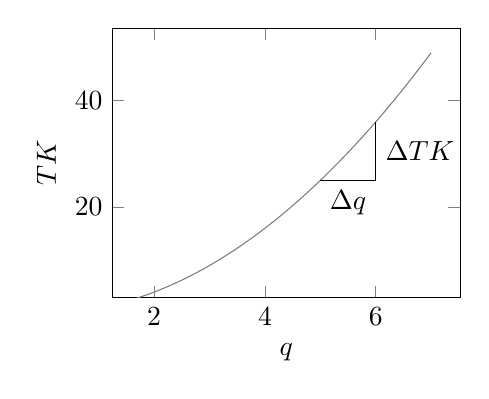
\begin{tikzpicture}
	\begin{axis}[name=left,xlabel=$q$, ylabel=$TK$, ymin=3,width=6cm, height=5cm]
		\addplot[gray, samples=100, domain=0:7] {x^2};
		\draw (axis cs:5,25) -- node[below]{$\Delta q$} (axis cs:6,25);
		\draw (axis cs:6,25) -- node[right]{$\Delta TK$} (axis cs:6,36);
	\end{axis}
\end{tikzpicture}
\caption{Hetzelfde als figuur \ref{fig:appendix1}, maar bij continue variatie}
\label{fig:appendix2}
\end{figure}

\subsection{Over het Begrip Logaritme}\label{sec:applog}

In hoofdstuk \ref{sec:h1bbp} werd een grafiek van het BBP van verscheidene regio's doorheen de tijd weergegeven. Hierbij werd er gebruik gemaakt van een logaritmische schaal. Wat is nu een \entry{logaritme}? Dat is een functie $log(x)$ die voor een bepaald getal de exponent geeft waarmee een constante waarde (het `grondtal') moet worden opgeheven om dat bepaalde getal als resultaat te bekomen. Bij de \entry{natuurlijke logaritme} is het grondtal $e=2,718281828...$\footnote{Een wiskundige constante ingevoerd door Leonhard Euler.}
\par De logaritme van een getal $x$ geeft dus de grootte-orde van $x$ aan. Als we als grondtal $10$ nemen, dan is de logaritme van $1$ gelijk aan $0$ (want $10^0=1$). Die van $10$ is $1$ (want $10^1=10$). Die van $100$ is $2$, die van $1000$ is $3$, enzovoort.\\

\par Bij het berekenen van economische groei komt de logaritme goed van pas. We kijken even naar het re\"eel BBP van een bepaald land op een bepaald tijdstip. We noteren dit als $Q_t$. De absolute verandering ten opzichte van het re\"eel BBP op een ander tijdstip ($Q_{t-1}$) is dan $\Delta Q_t=Q_t-Q_{t-1}$. De relatieve verandering, in procenten uitgedrukt, is gelijk aan $\frac{\Delta Q_t}{Q_{t-1}}\times 100$. Op jaarbasis ($t$ is dan een jaartal) noemt men dit de jaarlijkse \entry{groeivoet} $g$.\\

\par In hoofdstuk \ref{sec:h5groei} zagen we hoe we de gemiddelde jaarlijkse groeivoet berekent. We herhalen dit hier even. Voor de groei van een beginjaar $Y_0$ naar een ander jaar geldt :
$$Y_1=Y_0(1+g_1)$$
$$Y_2=Y_0(1+g_1)(1+g_2)=Y_0(1+g_g)^2$$
$$...$$
$$Y_n=Y_0(1+g_g)^n$$
Dus geldt voor de gemiddelde groeivoet $g_g$ :
$$(1+g_g)=\sqrt[n]{\frac{Y_n}{Y_0}}\qquad\Rightarrow\qquad g_g=\frac{Y_n}{Y_0}^{\frac{1}{n}}-1$$ 

\par Momenteel zijn we wel nog altijd aan het werken met groei over een bepaalde periode, zoals een jaar of meerdere jaren. Het niet-lineair groeiproces kan ook weergegeven worden in een continue vorm aan de hand van de volgende formule :
$$Q(t)=Q_0\cdot e^{g\cdot t}$$
Met $e$ het grondtal van de \entry{natuurlijke logaritme}. Nu is de groeivoet een `\textit{ogenblikkelijke groeivoet}' die geldt op elk moment in de tijd. De afgeleide (hoofdstuk \ref{sec:appafg}) is immers :
$$\frac{dQ(t)}{dt}=Q_0\cdot e^{g\cdot t}\cdot g=Q(t)\cdot g$$
En dus is de relatieve verandering gelijk aan :
$$\frac{\frac{dQ(t)}{dt}}{dt}{Q(t)}=g$$

\par Het voordeel van de continue formulering blijkt als we de logaritme nemen van $Q(t)$ :
$$\text{ln }Q(t)=\text{ln}\left(Q_0\cdot e^{g\cdot t}\right)=\text{ln }Q_0+g\cdot t$$
De logaritme van een product is gelijk aan de som van de logaritmen, en de natuurlijke logaritme heft het getal $e$ op. De resulterende vergelijking verschijnt als een rechte met richtingsco\"effici\"ent (stijging) $g$.
\par Op die manier kan men de groeivoet bij gegeven groei van het BBP schatten : men neemt de logaritme en dan kan de richtingsco\"effici\"ent visueel afgelezen worden. En die is gelijk aan $g$.
